\documentclass[twocolumn]{IEEEtran}
\usepackage[utf8x]{inputenc}
\usepackage{amssymb,amsfonts}
\usepackage[tbtags]{amsmath}
\usepackage{graphicx}
\usepackage{cite}
\usepackage{slashbox}
\usepackage{pict2e}
\usepackage{float}
\usepackage[all]{xy}
\usepackage{graphics,graphicx,color,colortbl}
\usepackage{times}
\usepackage{subfigure}
\usepackage{wrapfig}
\usepackage{multicol}
\usepackage{cite}
\usepackage{url}
\usepackage[tbtags]{amsmath}
\usepackage{amsmath,amssymb,amsfonts,amsbsy}
\usepackage{bm}
\usepackage{algorithm}
\usepackage{algorithmic}
\usepackage[centerlast, small]{caption}
\usepackage[colorlinks=true, citecolor=blue, linkcolor=blue, urlcolor=blue, breaklinks=true]{hyperref}
\begin{document}
\title{Circuitos acoplados magnéticamente}
\author{José Fabio Lozano Ovalle Código: $222982$\\
	Wilson Orlando Macias Fuquen Código: $223101$\\
	David Ricardo Martínez Hernández Código: $261931$}
\maketitle
\markboth{Universidad Nacional de Colombia}{}
\floatname{algorithm}{Algoritmo}
\begin{abstract}
Se realizara el montaje de un circuito acoplado magnéticamente y se hallaran experimentalmente los valores de $L_1$, $L_2$ y $M$, adicionalmente se determinara la polaridad relativa de los inductores y la relación de transformación entre primario y secundario. Por ultimo se implementara un circuito para  visualizar la curva de histéresis del núcleo de hierro utilizado para acoplar los inductores.
\end{abstract}
\begin{keywords}
Autoinductancia, Bobina, Corriente, Flujo Magnético, Histéresis, Inductancia Mutua, Magnetismo, Magnetización, Material Ferromagnético, Permeabilidad.
\end{keywords}

\section{Objetivos}
\begin{itemize}
 \item Visualizar experimentalmente el ciclo de histéresis del núcleo hierro utilizado como acople por medio del osciloscopio.
 \item Aplicar las ecuaciones de Ampere y Faraday en el planteamiento de las ecuaciones de los circuitos del sistema acoplado magnéticamente.
 \item Determinar experimentalmente los valores de $L_1$, $L_2$, $M$, y la polaridad relativa de los inductores.
 \item Comparar experimentalmente la relación de transformación entre primario y secundario, por medio del número de espiras, voltajes y corrientes.
\end{itemize}

\section{Introducción}
\noindent
Siempre que la corriente fluye a través de un conductor, ya sea $AC$ o $DC$, se genera un campo alrededor de él. En circuitos, se refiere a menudo al \textit{flujo magnético} a través de un lazo de alambre, que es la componente normal promedio del campo magnético que emana del lazo, multiplicada por el área del mismo. Cuando un campo magnético variable en el tiempo generado por un lazo penetra un segundo lazo, se induce una tensión entre los extremos de este último.\footnote{Texto tomado de \cite{hayt}, Página 491}

\section{Marco Teórico}
\subsection{Inductancia Mutua}
\noindent
Cuando $2$ inductores se encuentran muy cerca el uno del otro, el flujo magnético causado por la corriente en una bobina penetra la otra bobina, se induce una tensión en la segunda bobina, este fenómeno se conoce como \textbf{inductancia mutua}. Primero se considerara una bobina con $N$ vueltas, cuando la corriente $i$ se a través de la bobina, un flujo magnético $\phi$ se produce a su alrededor Fig. \ref{fig1},
\begin{figure}[H]
	\centering
		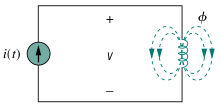
\includegraphics[scale=0.6]{flujomagnetico.png}
	\caption{Flujo magnético producido por una bobina simple con $N$ espiras (Imagen tomada de \cite{sadiku}, Página $528$)}
	\label{fig1}
\end{figure}
\noindent
de acuerdo a la ley de Faraday, la tensión inducida $v$ en la bobina es proporcional al número de vueltas $N$ y la razón de cambio del flujo magnético $\phi$, es decir:
\begin{equation}
 v = N \frac{d \phi}{d t}
\label{ecu1}
\end{equation}
\noindent
Pero el flujo $\phi$ es producido por la corriente $i$ de manera que cualquier cambio en $\phi$ es producido por un cambio en la corriente. Por lo tanto
\begin{equation}
 v = N \frac{d \phi}{d t}\frac{d i}{d t}\ \ o\ \ v = L \frac{d i}{d t}
\label{ecu2}
\end{equation}
\noindent
de la ecuación anterior se puede deducir que la inductancia $L$ de la bobina viene dada por
\begin{equation}
 L = N \frac{d \phi}{d i}
\label{ecu3}
\end{equation}
\noindent
Esta inductancia que comúnmente se llama \textit{autoinductancia}, porque se relaciona con la tensión inducida en una bobina por una corriente variable en el tiempo en la misma bobina.\\\\
Ahora se consideran 2 bobinas con autoinductancias $L_1$ y $L_2$ que están muy cerca entre sí Fig. \ref{fig2}, la bobina $1$ tiene $N_1$ espiras, mientras que la bobina $2$ tiene $N_2$ espiras. Por simplicidad se asume que la bobina $2$ no tiene corriente. El flujo magnético $\phi _1$ emanado por la bibina $1$ tiene dos componentes:
\begin{itemize}
 \item $\phi _{11}$ vinculado sólo por la bobina 1
 \item $\phi _{12}$ vinculado por ambas bobinas
\end{itemize}
\begin{figure}[H]
	\centering
		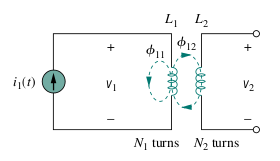
\includegraphics[scale=0.6]{2bobinas.png}
	\caption{Inductancias mutuas $M_{21}$ de la bobina $2$ con respecto a la bobina $1$ (Imagen tomada de \cite{sadiku}, Página $529$)}
	\label{fig2}
\end{figure}
\begin{equation}
 \phi _1 = \phi _{11} + \phi _{12} 
\label{ecu4}
\end{equation}
\noindent
A pesar de las dos bobinas están físicamente separadas, se dice que son \textit{magnéticamente acopladas}. El voltaje inducido en la bobina $1$
\begin{equation}
 v_1 = N_1 \frac{d \phi _1}{d i_t}
\label{ecu5}
\end{equation}
\noindent
Sólo el flujo $\phi _{12}$ vinculado a la bobina $2$, entonces la tensión inducida en la bobina $2$
\begin{equation}
 v_2 = N_2 \frac{d \phi _{12}}{d i_t}
\label{ecu6}
\end{equation}
\noindent
Nuevamente, como los flujos son causados ​​por la corriente $i_1$ que fluye en la bobina $1$, la ecu. (\ref{ecu5}) se puede escribir como
\begin{equation}
 v_1 = N_1 \frac{d \phi _1}{d i_1} \frac{d i_1}{dt} = L_1 \frac{d i_1}{d t}
\label{ecu7}
\end{equation}
\noindent
donde $L_1 = N_1\frac{d \phi _{1}}{d i_1}$ es la autoinductancia de la bobina $1$. De manera similar la ecu. (\ref{ecu6}) se puede escribir como
\begin{equation}
 v_2 = N_2 \frac{d \phi _{12}}{d i_1} \frac{d i_1}{dt} = M_{21} \frac{d i_1}{d t}
\label{ecu8}
\end{equation}
\noindent
donde
\begin{equation}
 M_{21} = N_2 \frac{d \phi _{12}}{d i_1}
\label{ecu9}
\end{equation}
\noindent
$M_{21}$ es conocida como la inductancia mutua de la bobina $2$ con respecto a la bobina $1$. El subíndice $21$ indica que la inductancia de la $M_21$ se relaciona la tensión inducida en la bobina $2$ de la corriente en la bobina $1$. Por lo tanto, la tensión mutua de circuito abierto (o voltaje inducido) a través de la bobina $2$ es
\begin{equation}
 v_2 = M_{21} \frac{d i_1}{d t}
\label{ecu10}
\end{equation}
\noindent
Ahora se supone que la corriente $i_2$ circula en la bobina $2$, mientras que la bobina $1$ no lleva corriente Fig. \ref{fig3}
\begin{figure}[H]
	\centering
		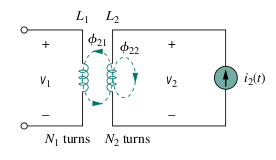
\includegraphics[scale=0.6]{2bob.png}
	\caption{Inductancias mutuas $M_{12}$ de la bobina $2$ con respecto a la bobina $2$ (Imagen tomada de \cite{sadiku}, Página $529$)}
	\label{fig3}
\end{figure}
\noindent
El flujo magnético $\phi _2$ que emana de la bobina $2$ comprende el flujo $\phi _{22}$ que une sólo la bobina $2$ y el flujo $\phi _{21}$ que conecta las dos bobinas. Por lo tanto,
\begin{equation}
 \phi _2 = \phi _{21} + \phi _{22}
\label{ecu11}
\end{equation}
\noindent
La entrada del flujo $\phi _2$, por lo que la tensión inducida en la bobina $2$ es
\begin{equation}
 v_2 = N_2 \frac{d \phi _2}{d t} = N_2 \frac{d \phi _2}{d i_2} \frac{d i_2}{d t} = L_2 \frac{d i_2}{d t}
\label{ecu12}
\end{equation}
\noindent
donde $L_2 = N_2 \frac{d \phi _2}{d i_2}$ es la inductancia mutua de la bobina $2$. Siendo solo el flujo $\phi _{21}$ vinculado de la bobina $1$, el voltaje inducido en la bobina $1$ es
\begin{equation}
 v_1 = N_1 \frac{d \phi _{21}}{d t} = N_1 \frac{d \phi _{21}}{d i_2} \frac{d i_2}{d t} = M_{12} \frac{d i_2}{d t}
\label{ecu13}
\end{equation}
\noindent
donde
\begin{equation}
 M_{12} = N_1 \frac{d \phi _{21}}{d i_2}
\label{ecu14}
\end{equation}
\noindent
que es la inductancia mutua de la bobina $1$ con respecto a la bobina $2$. Por lo tanto, la tensión de circuito abierto a través de la bobina $1$ es
\begin{equation}
 v_1 = M_{12} \frac{d i_2}{d t}
\label{ecu15}
\end{equation}
\begin{equation}
 M_{12} = M_{21} = M
\label{ecu16}
\end{equation}
\noindent
$M$ es la inductancia mutua entre las dos bobinas. Al igual que autoinductancia $L$, inductancia mutua $M$ se mide en henrios ($H$). Tenga en cuenta que el acoplamiento mutuo sólo existe cuando los inductores o bobinas están muy cerca, y los circuitos son impulsados ​​por fuentes variables en el tiempo.\\
De los dos casos en las Fig. \ref{fig2} y \ref{fig3}, se concluye que los resultados de la inductancia mutua si un voltaje es inducido por una corriente variable en el tiempo en otro circuito. Es la propiedad de un inductor para producir un voltaje en respuesta a una corriente variable en el tiempo en otro inductor cerca de él.\\\\
A pesar de la inductancia mutua $M$ es siempre una cantidad positiva, la tensión mutua $M\ \ di / dt$ puede ser negativo o positivo, al igual que la tensión autoinducida $L\ \ di / dt$. Sin embargo, a diferencia del auto-inducido $L\ \ di/ dt$, cuya polaridad es determinado por la dirección de la corriente de referencia y la polaridad de la tensión de referencia (de acuerdo con la convención de signos pasiva), la polaridad de la tensión mutua $M\ \ di / dt$ no es fácil de determinar, debido a que cuatro terminales están involucradas.\\
La elección de la polaridad correcta para $M\ \  di / dt$ se hace mediante el examen de la forma o la orientación particular en la que las dos bobinas están físicamente separadas y la aplicación de la ley de Lenz en relación con la regla de la mano derecha. Ya que es un inconveniente para mostrar los detalles de construcción de las bobinas en un esquema del circuito, se aplica la convención del punto en el análisis de circuitos.\\
Por esta convención, un punto se coloca en el circuito en un extremo de cada una de las dos bobinas con acoplamiento magnético para indicar la dirección del flujo magnético si la corriente entra en la terminal de puntos de la bobina. En la Fig. \ref{fig4} se observa dicha convención.
\begin{figure}[H]
	\centering
		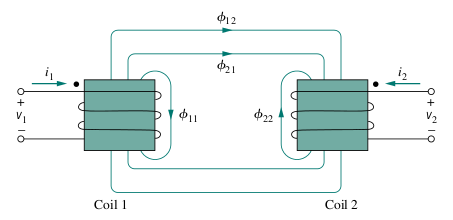
\includegraphics[scale=0.6]{point.png}
	\caption{Ilustración convención de puntos (Imagen tomada de \cite{sadiku}, Página $531$)}
	\label{fig4}
\end{figure}
\noindent
La convención del punto dice lo siguiente:\\
Si una corriente \textbf{entra} en la terminal de un punto de una bobina, la polaridad de la tensión de referencia mutua en la segunda bobina es \textbf{positiva},  si  entra en la terminal de puntos de la segunda bobina.\\
Por lo tanto, la polaridad de la tensión de referencia mutua depende de la dirección de referencia de la corriente de inducción y los puntos sobre las bobinas acopladas.\\
La aplicación de la convención del punto se ilustra en los cuatro pares de bobinas acopladas mutuamente Fig. \ref{fig5}.
\begin{figure}[H]
 \centering
    \subfigure[]{\label{fig5a}
      \fbox{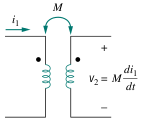
\includegraphics[scale=0.7]{pointsa.png}}}
  \hspace{0.5cm}
    \subfigure[]{\label{fig5b}
      \fbox{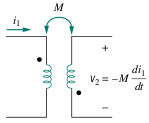
\includegraphics[scale=0.7]{pointsb.png}}}
  \hspace{0.5cm}
    \subfigure[]{\label{fig5c}
      \fbox{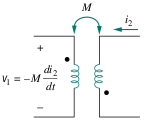
\includegraphics[scale=0.7]{pointsc.png}}}
  \hspace{0.5cm}
    \subfigure[]{\label{fig5d}
      \fbox{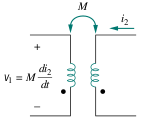
\includegraphics[scale=0.7]{pointsd.png}}}
  \caption{Convención de puntos (Imagen tomada de \cite{sadiku}, Página $531$)}
    \label{fig5}
\end{figure}
\noindent
La figura \ref{fig6} muestra la convención del punto de bobinas acoplados en serie.
\begin{figure}[H]
 \centering
    \subfigure[Conexión de Adición]{\label{fig6a}
      \fbox{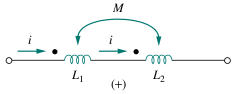
\includegraphics[scale=0.6]{currentpointa.png}}}
  \hspace{1cm}
    \subfigure[Conexión de Oposición]{\label{fig6b}
      \fbox{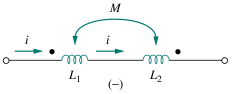
\includegraphics[scale=0.6]{currentpointb.png}}}
  \caption{Polaridad del voltaje con respecto a la convención de puntos (Imagen tomada de \cite{sadiku}, Página $532$)}
    \label{fig6}
\end{figure}
\noindent
\noindent
Para las bobinas de la figura. \ref{fig6a}, la inductancia total es
\begin{equation}
 L = L_1 + L_2 + 2M\ \ \ Conexion\ \ Aditiva
\label{ecu17}
\end{equation}
\noindent
para la bobina de la Fig. \ref{fig6b}
\begin{equation}
 L = L_1 + L_2 - 2M\ \ \ Conexion\ \ De\ \ Oposicon
\label{ecu18}
\end{equation}

\subsection{Coeficiente de Acoplamiento}
\noindent
El grado con el cual $M$ se acerca a su valor máximo se describe mediante el \textbf{coeficiente de acoplamiento}.\footnote{Texto tomado de \cite{hayt}}

\begin{equation}
 k = \frac{M}{\sqrt{L_1 L_2}}
\label{ecu19}
\end{equation}
\noindent
Puesto que $M \le \sqrt{L_1L_2}$
$$0 \le k \le 1$$
\noindent
Los valores más grandes del coeficiente de acoplamiento se obtiene con bobinas que están físicamente más próximas, o que tienen un núcleo de alta permeabilidad. Se dice que las bobinas que tienen un coeficiente de acoplamiento cercano a la unidad están \textbf{estrechamente acopladas}\footnote{Texto tomado de \cite{hayt}, Página $502$}.

\section{Hipótesis}
\noindent
Se espera que la relación de transformación sea muy parecida a la razón del número de espiras entre secundario  y primario.\\
Se espera una curva de histéresis de área pequeña si el núcleo no se calienta demasiado, de lo contrario se tendría una curva un poco mas ancha.

\section{Materiales}
\begin{itemize}
 \item Bobinas
 \item Condensador de $1\ \ \mu F$
 \item Multímetro
 \item Núcleo de un material Ferromagnético
 \item Osciloscopio
 \item Resistencias
\end{itemize}

\section{Análisis Y Resultados}
\noindent
Para esta práctica se implementaran 2 circuitos monofásico para analizar en estos el fenómeno de acoplamiento magnético.

\subsection{Circuito con transformador }
\noindent
Para este circuito se tiene una fuente AC que alimenta el primario y en el secundario se tiene un circuito abierto para analizar la tensión en cada uno y obtener la ganancia del transformador.
\begin{figure}[H]
	\centering
		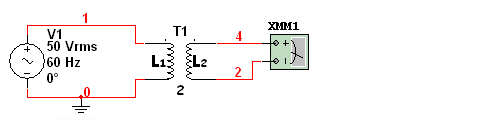
\includegraphics[scale=0.7]{circ1.PNG}
	\caption{Circuito monofásico con transformador.}
	\label{fig10}
\end{figure}

\subsubsection{Relación de transformación}
\noindent
Para este circuito se tiene  una tensión en $L_1$ de $V_1$=50[V], y en $L_2$ un $V_2$=25[V]aproximadamente, con estos datos se obtiene una relación de transformación debido a la tensión en el primario con respecto secundario.
\begin{equation}
 m =  \frac{V_1}{V_2}=\frac{50[V]}{25[V]}=2
\label{ecu30}
\end{equation}
\noindent
Esto se comprobara en la práctica con la relación en el número de espiras en cada embobinado así:
\begin{equation}
 m =  \frac{N_2}{N_2}
\label{ecu31}
\end{equation}

\subsubsection{Procedimiento para calcular inductancias $L_1$, $L_2$ y $m$}
\noindent
Para obtener los valores de $L_1$, $L_2$ y $M$ se tiene datos como la corriente $i_1(T)$ y sabiendo que:
\begin{equation}
 V_1=jwL_1i_1
\label{ecu50}
\end{equation}
\noindent
Donde se despeja y se obtiene:
\begin{equation}
 L_1=\frac{V_1}{jw i_1}
\label{ecu51}
\end{equation}
\noindent
De igual manera se puede tener obtener $L_2$ intercambiando la energización de la fuente $AC$, además M se obtiene así:
\begin{equation}
 M=\frac{V_2}{jw i_1}
\label{ecu52}
\end{equation}

\subsubsection{Procedimiento para hallar la polaridad relativa de los devanados primario y secundario}
\noindent
Para esta parte se debe hacer un cambio en el circuito original, se debe hacer una conexión entre las tierras de los circuitos acoplados magnéticamente, este circuito queda así:
\begin{figure}[H]
	\centering
		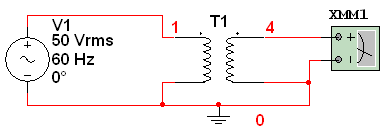
\includegraphics[scale=0.6]{circ3.PNG}
	\caption{Circuito para polaridad relativa.}
	\label{fig12}
\end{figure}
\noindent
Luego se mide la tensión entre los puntos restantes, en el circuito de la Fig.\ref{fig12} entre los puntos 1 y 4, a esta tensión se le llamara $V$, si se tiene que
\begin{equation}
 V=V_1-V_2
\label{ecu53}
\end{equation}
La polaridad de los devanados, es decir la convención de punto es tal como está en el circuito de la Fig.\ref{fig10}, si no, entonces se tiene que
\begin{equation}
 V=V_1+V_2
\label{ecu54}
\end{equation}
\noindent
Y la polaridad del circuito es diferente, en el segundo devanado el punto se ubica en el otro extremo.

\subsection{Circuito para obtener curva de histéresis}
\noindent
Para obtener la curva de histéresis del núcleo en el transformador, en este caso un material ferromagnético, se diseña el siguiente circuito.
\begin{figure}[H]
	\centering
		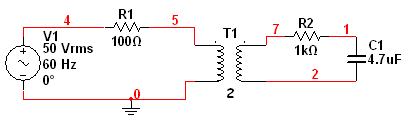
\includegraphics[scale=0.6]{circ2.PNG}
	\caption{Circuito para obtener curva de histéresis.}
	\label{fig11}
\end{figure}
\noindent
Para obtener la curva se tiene que la tensión en el condensador es
\begin{equation}
V_c(t)=\frac{1}{C}\displaystyle\int_{0}^{t} i_c(\tau)\, d\tau
\label{ecu32}
\end{equation}
\noindent
Donde $i_c(t)$ es la corriente en $R_2$ y $L_2$, entonces se tiene:
\begin{equation}
i_c(t)=\frac{V_2(t)}{R_2}
\label{ecu33}
\end{equation}
\noindent
Donde $V_2(t)$ es la tensión en el secundario, además con la ley de Faraday se puede relacionar esta tensión con el flujo en el núcleo:
\begin{equation}
V_2(t)=N_2\frac{d \phi(t)}{dt}
\label{ecu34}
\end{equation}
\noindent
Recordando que:
\begin{equation}
\phi(t)=A B(t)
\label{ecu35}
\end{equation}
\noindent
Así se obtiene que la tensión en el secundario está dada por:
\begin{equation}
V_2(t)=AN_2\frac{dB(t)}{dt}=i_c(t)R_2
\label{ecu36}
\end{equation}
\noindent
Reemplazando en la ecuación  \ref{ecu32} se obtiene que:
\begin{equation}
V_c(t)=\frac{AN_2}{CR_2}\displaystyle\int_{0}^{t} \frac{dB(\tau)}{d\tau}\, d\tau=\frac{AN_2B(\tau)}{CR_2}\
\label{ecu37}
\end{equation}
\noindent
De donde podemos obtener $B(t)$ de forma indirecta:
\begin{equation}
B(t)=\frac{CR_2 V_c(t)}{AN_2}
\label{ecu38}
\end{equation}
\noindent
Ahora, $H(t)$ se obtiene a partir de la ley de Ampere:
\begin{equation}
\displaystyle\oint_{C} H(t)\, dl=H(t)l_m=N_1i_1(t)
\label{ecu39}
\end{equation}
\noindent
Despejando $H(t)$ se obtiene
\begin{equation}
H(t)=\frac{N_1i_1(t)}{l_m}
\label{ecu40}
\end{equation}
\noindent
Además, se sabe que la corriente  $i_1$, del primario es:
\begin{equation}
i_1(t)=\frac{V_{R1}}{R_1}
\label{ecu41}
\end{equation}
\noindent
Así se obtiene finalmente:
\begin{equation}
H(t)=\frac{N_1V_{R1}}{R_1l_m}
\label{ecu42}
\end{equation}
\noindent
Se puede observar en la ecuación \ref{ecu38} y  \ref{ecu42} que $B(t)$ y $H(t)$ dependen de $V_c(t)$ y $V_{R1}$ respectivamente, además de un valor contante dado por las características del circuito, midiendo la tensión de estos elementos con un osciloscopio y programándolo en la forma $XY$ se obtendrá finalmente la curva de histéresis.

\section{Preguntas}
\begin{enumerate}
 \item ¿Como se pueden hallar los valores de $L$ y $M$ en una inductancia a partir de $V$ e $I$?\\
Para calcular los valores de $L_1$, $L_2$ y $M$ en el circuito utilizando las mediciones de corriente y voltaje montamos el siguiente circuito, donde el secundario permanece abierto Fig. \ref{fig5a}.\\
De la malla del circuito dos en el dominio de la frecuencia obtenemos la ecuación:
\begin{equation}
 V_2 = j \omega Mi_1
\label{equ1}
\end{equation}
\noindent
Donde podemos despejar el valor de M ya que conocemos $i_1$ y $V_2$.
Ahora realizando la malla del circuito uno en el dominio de la frecuencia obtenemos:
\begin{equation}
 {V_1} = j\omega {L_1}{i_1} + j\omega M{i_2}
\label{equ2}
\end{equation}
\noindent
Como la corriente $i_2$ es cero entonces el valor de $L_1$ se puede calcular fácilmente de la expresión:
\begin{equation}
 {V_1} = j\omega {L_1}{i_1}
\label{equ3}
\end{equation}
\noindent
Por ultimo para encontrar el valor de $L_2$ cerramos el circuito para obtener la malla:
\begin{equation}
 {V_2} = j\omega {L_2}{i_2} + j\omega M{i_1}
\label{equ4}
\end{equation}
\noindent
Donde ya son conocidos todos los valores, entonces podemos despejar $L_2$

 \item ¿Como se aplica la ley de Ampere y la ley de Faraday a un circuito de acoplamiento magnético?\\
En un circuito acoplado magnéticamente donde circula una corriente $i_1$ y el inductor $L_1$ tiene $N$ espiras, longitud $l$ y área $S$. Aplicando la ley de Ampere podemos hallar el flujo magnético en la bobina $L_1$, multiplicando el campo magnético por el área $S$:
\begin{equation}
{\Phi _1} = S{B_1} = \frac{{{\mu _0}NS{i_1}}}{l}
\label{equ5}
\end{equation}
\noindent
Si las dos bobinas tienen la misma área $S$ el flujo magnético que pasa por la segunda bobina es el mismo que genera la primera.\\
Podemos hallar el coeficiente $M$ de inducción mutua, que es la relación del flujo que pasa por la segunda bobina y la corriente que pasa por la primera.
\begin{equation}
 M = \frac{{{\Phi _2}}}{{{i_1}}} = \frac{{{\mu _0}NS}}{l}
\label{equ6}
\end{equation}
\noindent
Aplicando la ley de Faraday para cuando la corriente $i_1$ varia en el tiempo se induce una $FEM$ en el circuito dos, que la podemos hallar derivando el flujo que atraviesa la bobina $L_2$, así hallamos $V_2$:
\begin{equation}
 {V_2} =  - \frac{{d{\Phi _2}}}{{dt}} =  - M\frac{{d{i_1}}}{{dt}}
\label{equ7}
\end{equation}

 \item ¿Que es la histéresis de un material ferromagnético y como se puede observar?\\
El ciclo de histéresis de un material ferromagnético se presenta cuando un campo magnético variable en el tiempo que puede ser generado por una corriente alterna sobre un inductor,  atraviesa el material, haciendo que sus dominios magnéticos estén en constante movimiento, ya que tienden a orientarse en la dirección del campo magnético inducido por la bobina. Representando el campo magnético en función de la densidad de campo magnético (que es proporcional a la corriente), obtenemos la curva de histéresis para un material ferromagnético.
\begin{figure}[H]
	\centering
		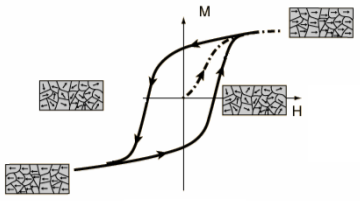
\includegraphics[scale=0.5]{pre3a.png}
	\caption{Curva de Histéresis}
	\label{fig100}
\end{figure}
\noindent
Para observar la curva de histéresis podemos utilizar un osciloscopio de dos canales en el modo $XY$, a continuación se muestra la conexión.
\begin{figure}[H]
	\centering
		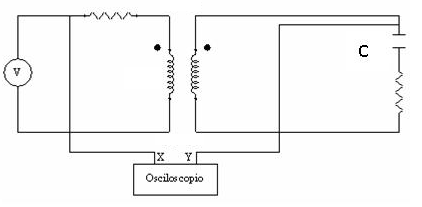
\includegraphics[scale=0.5]{pre3b.png}
	\caption{Conexión con el osciloscopio para visualizar la curva de histéresis}
	\label{fig101}
\end{figure}
\noindent
Donde  el voltaje  medido en $X$ es proporcional a la intensidad de campo magnético y el voltaje medido en $Y$ es proporcional a la densidad de flujo magnético.
\end{enumerate}

\bibliographystyle{ieeetran}
\begin{thebibliography}{99}
\bibitem{sadiku} Alexander, Charles K. \&  Sadiku, Matthew N.O.
{\em ```Fundamentals of Electric Circuits"'}.
McGRAW-HILL, ISE Editions, 1999.

\bibitem{dorf} Dorf  \& Svoboda.
{\em ```Circuitos Eléctricos"'}.
Alfaomega, Sexta Edición, 2006.

\bibitem{hayt} Hayt, William H. Jr., Kemmerly, Jack E. \& Durbin, Steven M.
{\em ```Análisis de circuitos en ingeniería"'}.
McGRAW-HILL, Séptima Edición, 2007.

\bibitem{nahvi} Nahvi, Mahmood \& Edminister, Joseph A.
{\em ```Theory and Problems of Electric Circuits"'}.
McGRAW-HILL, Fourth Edition, 2003.

\end{thebibliography}
\end{document}